\chapter{Results}
\label{ch:results}


The results obtained from the credit card fraud detection system give evidence of how well sophisticated deep learning models work for predicting unauthorized transactions. Four distinct machine-learning techniques were taught to distinguish between authentic and fraudulent transactions in this investigation. Accuracy and F1 score, which are crucial metrics for evaluating classification ability, differ throughout the models. A dataset with a variety of transactional anomalous patterns in which the models used to detect fraud transactions are Logistic Regression, Random Forest Classification, XGBoost model, and Cat Boost which can be utilized by importing the Python libraries, Scikit-learn, and xgboost. Each model is trained on the training data provided by the network and then tested against the testing data. After training these models, their performance is evaluated based on various evaluation metrics such as confusion matrix, accuracy score and F1 score. However, for this study, the F1 score is a more reliable measure to analyze the model’s efficiency than the accuracy score because of the imbalance in data as there are a large number of valid transactions and very few fraud transactions. 



 \begin{figure}[ht]
    \centering
    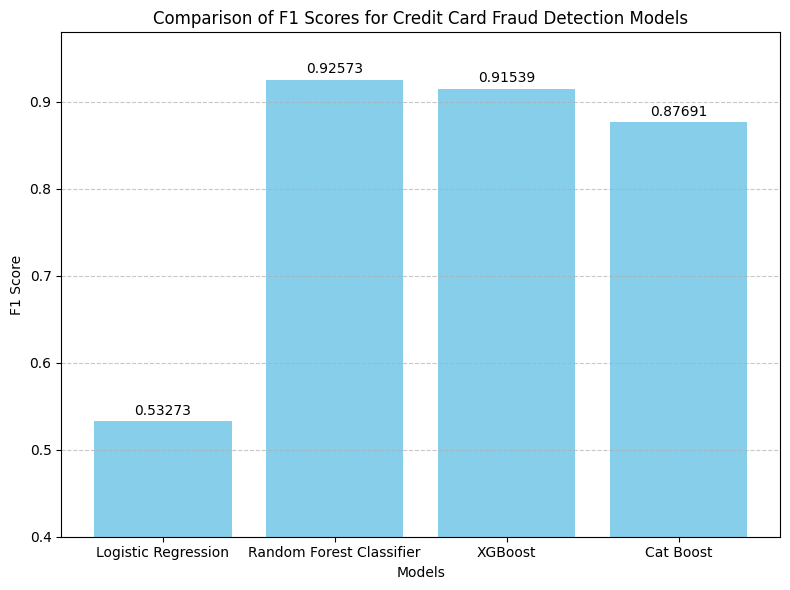
\includegraphics[scale=0.5]{figures/FinalPlot.png}
    \caption{Comparison of F1 Scores}
    \label{fig:Data Preprocessing}
\end{figure}
\clearpage


A bar plot visualization was utilized to compare the F1 scores, which indicates the Comparison of the F1 Scores of the four models. The graph showed that, in comparison to the other models, the Random Forest model performed the best and obtained the greatest F1 score.

This graphical representation made it very evident how much better the Random Forest model performed when detecting fraudulent transactions in the credit card system. These results demonstrate how important machine learning algorithms are in enhancing financial institutions' security against the constant danger of fraudulent activity. 


...





\section{Summary}






